\section{Conservation}

We expect the following quantities to be physically conserved: mass h, momentum or mass velocity, $hu$ and $hv$, and
energy 0.5($hv^2$+$gh^2$). Potential vorticity is only looked at in the 2D solver. 

\subsection{1D Conservation Laws}
Investigation of conservation laws in the 1D solver shows differences
between the conserved quantities Figure~\ref{fig:1D_cons}. The mass is hypothetically guessed to be strictly conserved by the scheme, along with 
momentum, unless there are reflections from the boundary conditions where the walls take some of the momentum. As we see from the energy conservation 
graph ''jumps'' at the time of shock formation Figure~\ref{fig:1D_cons}. We find energy is not conserved 
adequetly due to the inherent nature of the numerical schemes inability to capture solutions at the non-linear shocks \cite{Lax}. 
\newline

\begin{figure}[h!]
    \centering
    \begin{subfigure}[b]{0.9\textwidth}
        \centering
        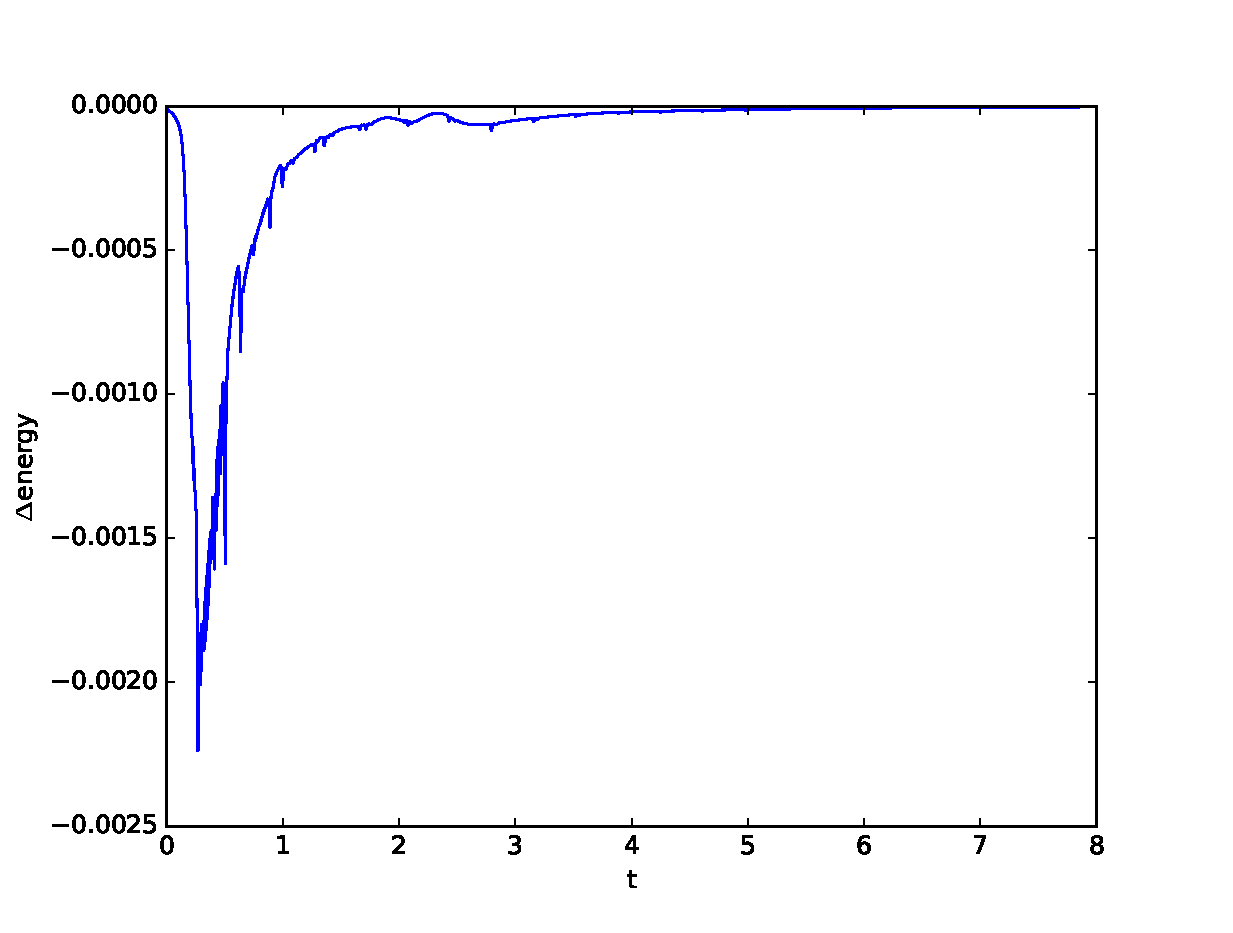
\includegraphics[width=1.1\textwidth,height=0.52\textwidth]{images/E1d.eps}\hfill
        \caption{Energy}
        \label{fig:Energy}
    \end{subfigure}
    \hfill
    \begin{subfigure}[b]{0.9\textwidth}
        \centering
        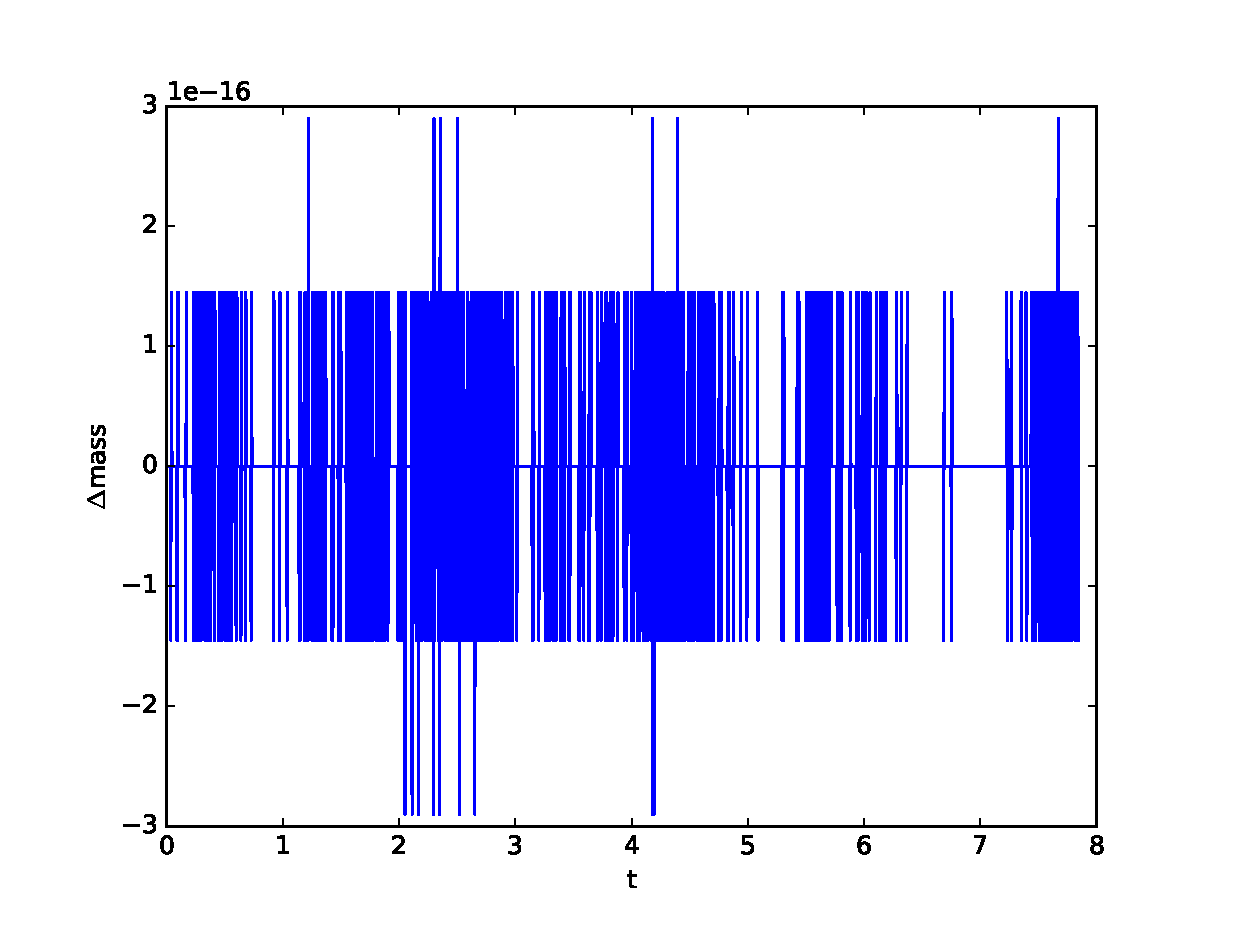
\includegraphics[width=1.1\textwidth, height=0.52\textwidth]{images/Ma1d.eps}\hfill
        \caption{Mass}
        \label{fig:Mass}
    \end{subfigure}
    \hfill
    \begin{subfigure}[b]{0.9\textwidth}
        \centering
        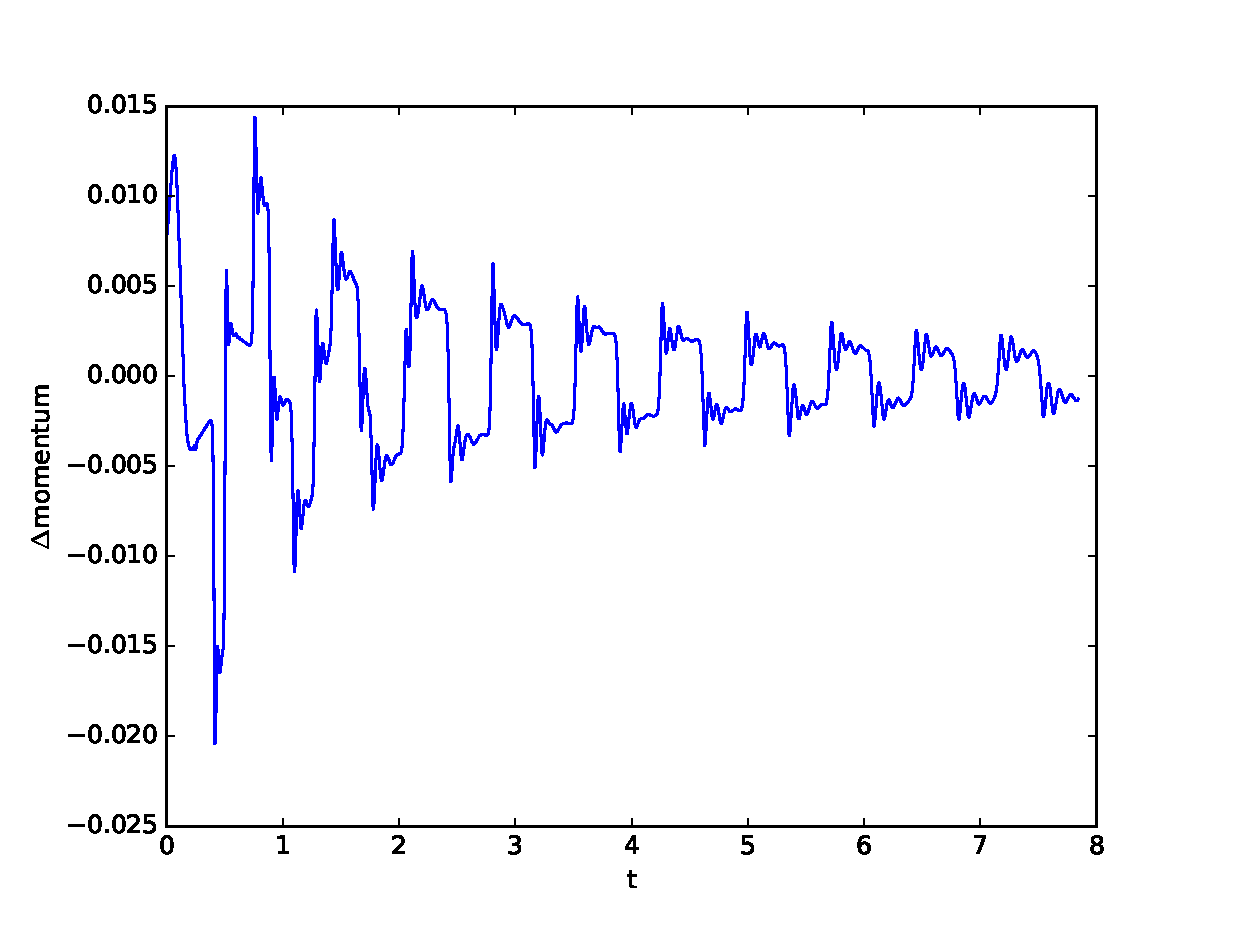
\includegraphics[width=1.1\textwidth,height=0.52\textwidth]{images/Mo1d.eps}\hfill
        \caption{Momentum}
        \label{Momentum}
    \end{subfigure}
    \caption{1D conservation plots.}
    \label{fig:1D_cons}
\end{figure}

\subsection{2D Conservation Laws}

In the 2D scheme the conserved quantities are again hypothetically guessed to be strictly conserved. The conservation laws
are analyzed using the two-step Richtmeyer 2D solver and show similar discrepencies
failing to show the energy is adequetly conserved Figure~\ref{fig:2Dcons_A}. 
The energy conservation is shown to suffer from the same flaws in the numerical scheme as before, and does not initially conserve
energy with the error of second order, similar to 1D. This leads to the same
presumption given for the 1D case. 
\newline

\begin{figure}[h!]
    \centering
    \begin{subfigure}[b]{0.9\textwidth}
        \centering
        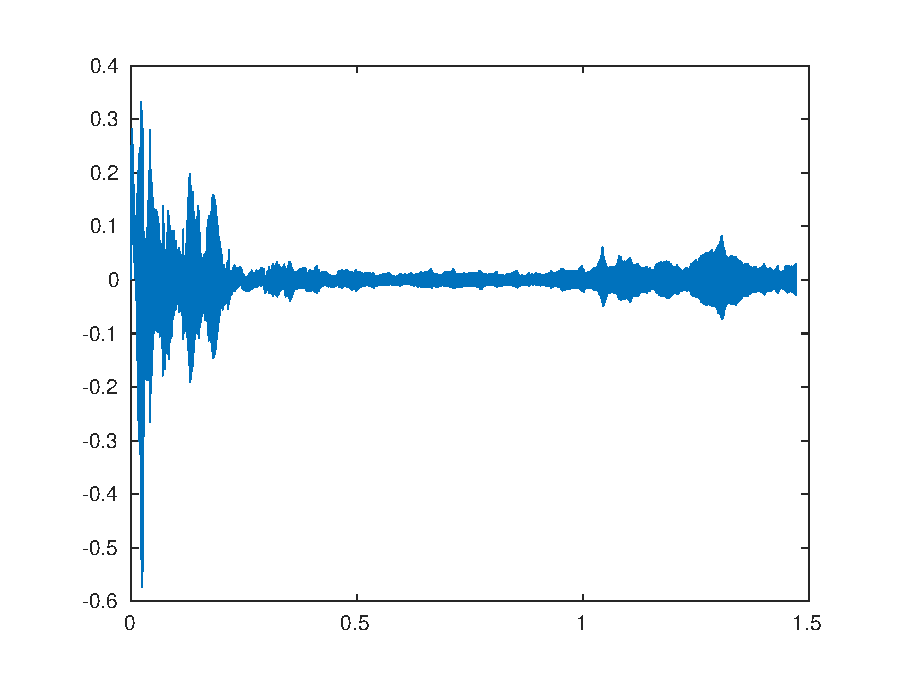
\includegraphics[width=1.1\textwidth,height=0.52\textwidth]{images/cons_energy.eps}\hfill
        \caption{Energy}
        \label{fig:Energy}
    \end{subfigure}
    \hfill
    \begin{subfigure}[b]{0.9\textwidth}
        \centering
        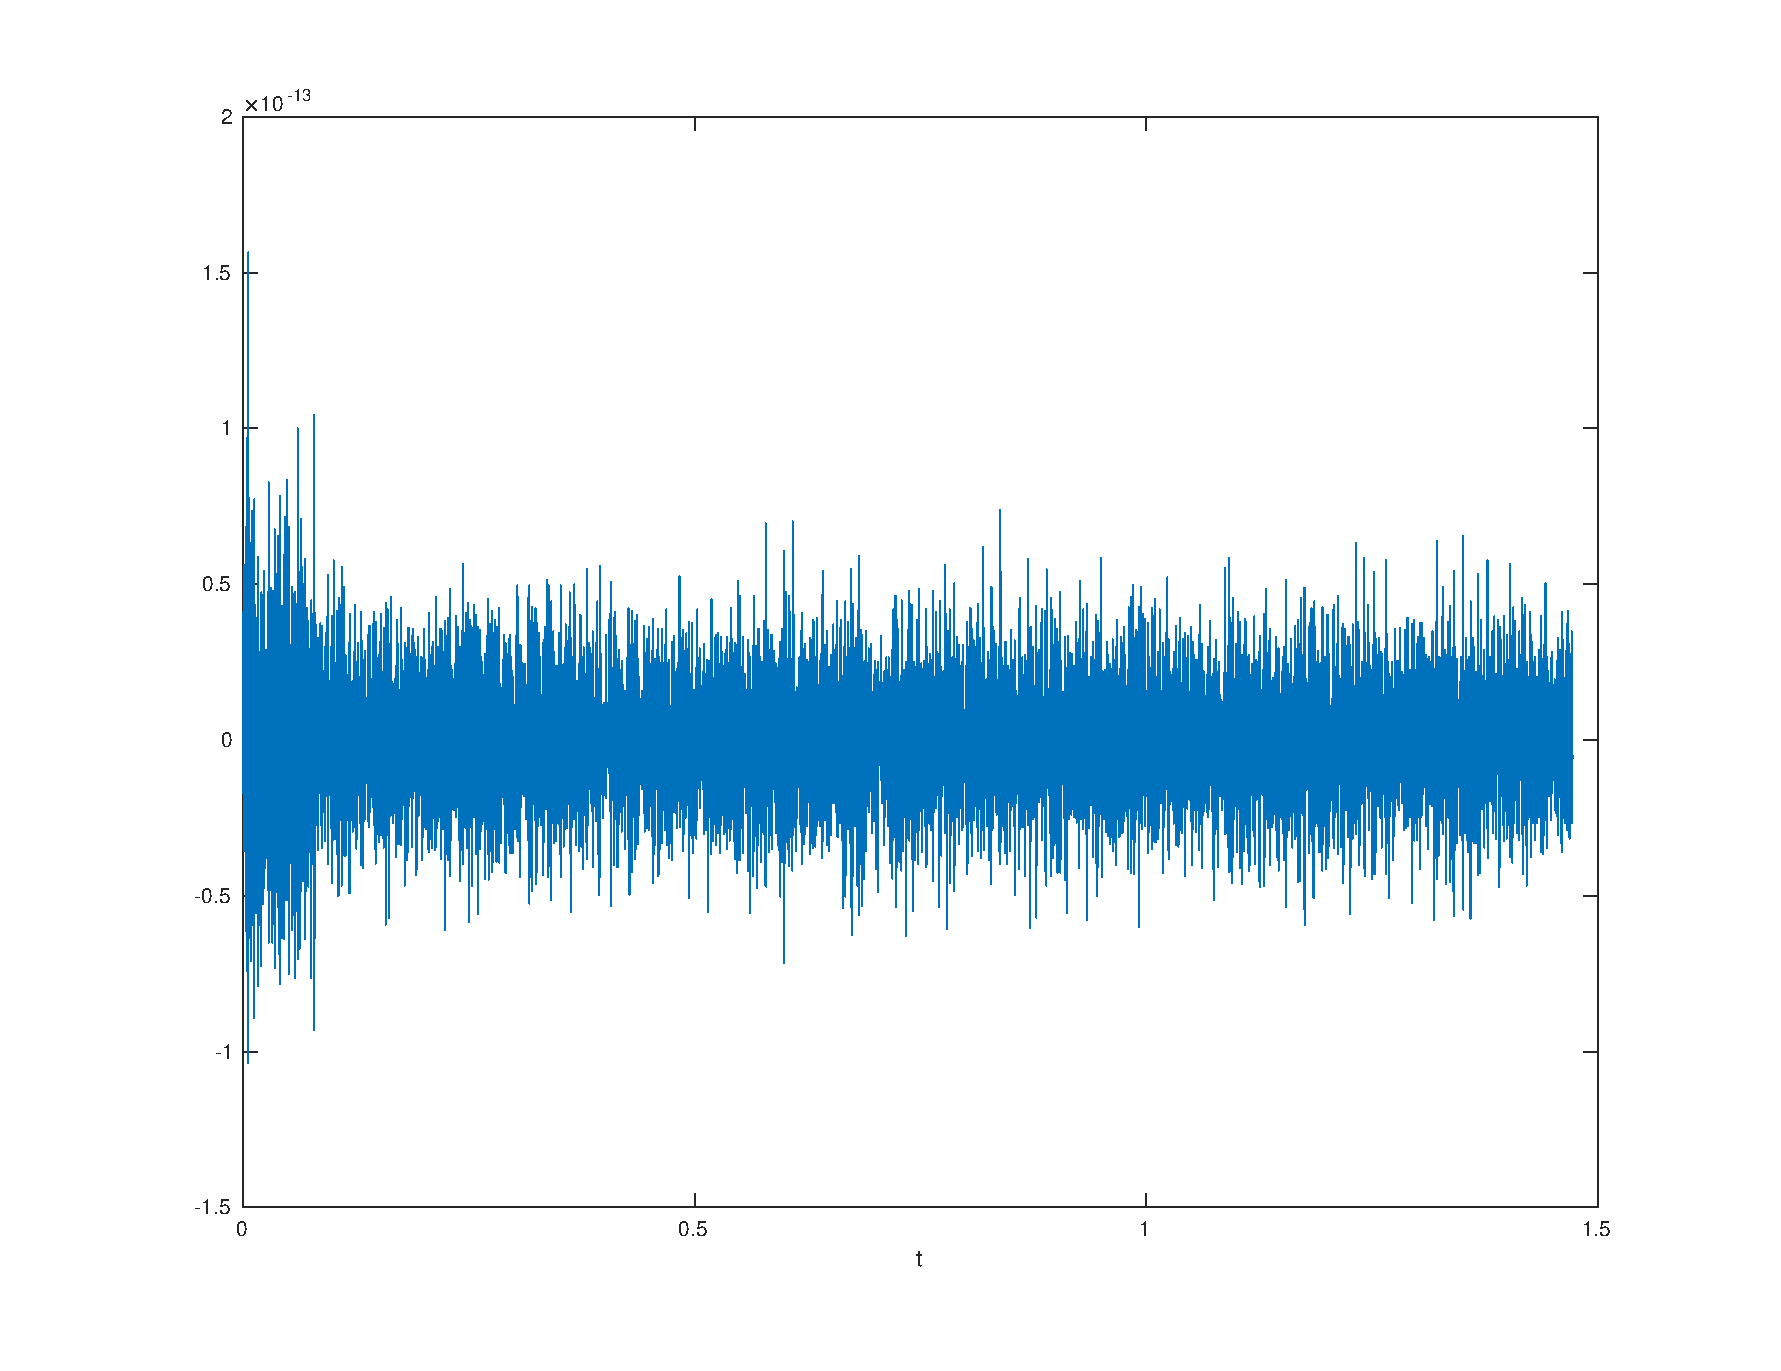
\includegraphics[width=1.1\textwidth, height=0.52\textwidth]{images/cons_mass.eps}\hfill
        \caption{Mass}
        \label{fig:Mass}
    \end{subfigure}
    \hfill
    \caption{2D conservation plots of mass and energy.}
    \label{fig:2Dcons_A}
\end{figure}


The potential vorticity is given by this formula,
\begin{equation}\label{eqn:13}
\frac{\partial hv}{\partial x} - \frac{\partial hu}{\partial y} 
\end{equation}
and should be conserved. We show potential vorticity to be conserved by using the 2D two-step method
of Richtmeyer Figure~\ref{fig:2Dcons_B}.
\newline

\begin{figure}[h!]
    \centering
    \begin{subfigure}[b]{0.9\textwidth}
        \centering
        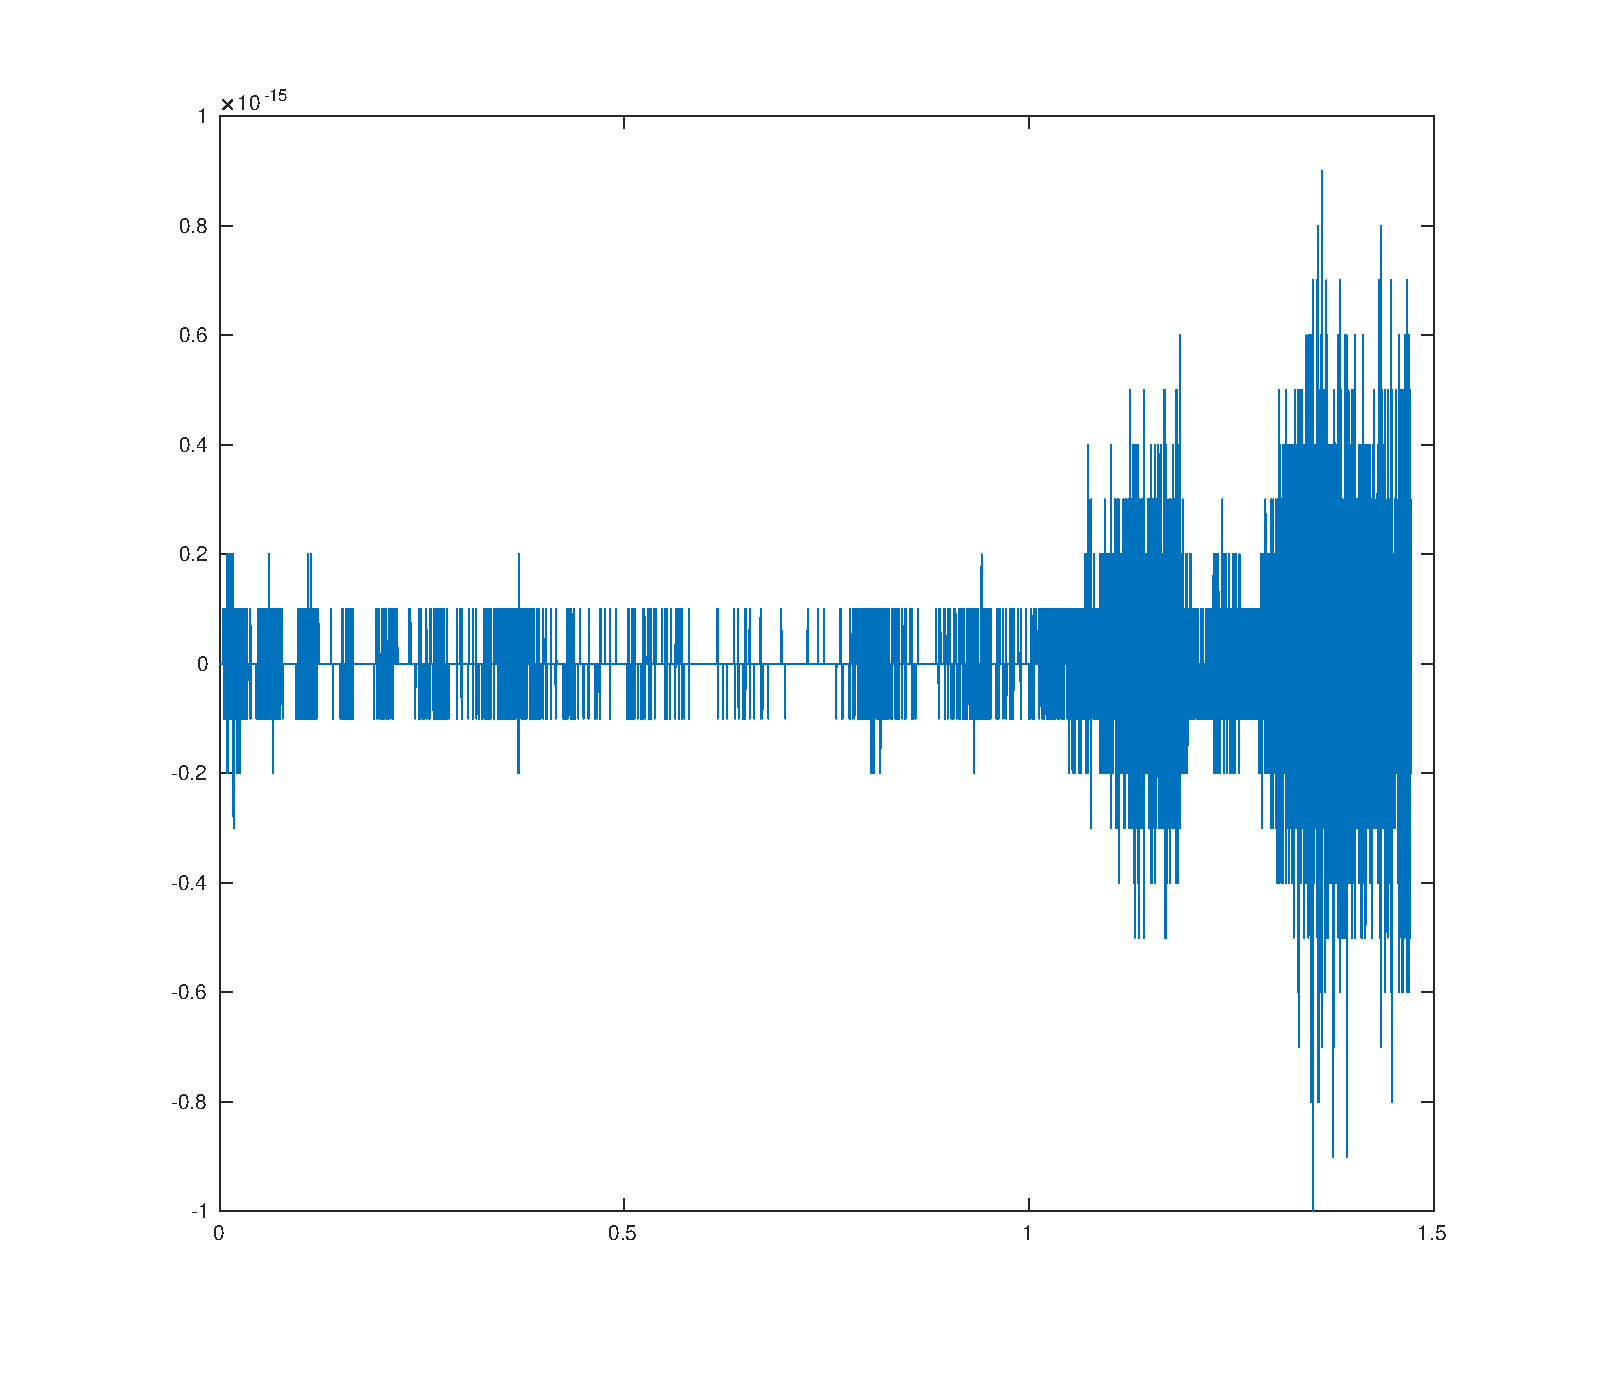
\includegraphics[width=1.1\textwidth,height=0.52\textwidth]{images/cons_momu.eps}\hfill
        \caption{u-momentum}
        \label{fig:Energy}
    \end{subfigure}
    \hfill
    \begin{subfigure}[b]{0.9\textwidth}
        \centering
        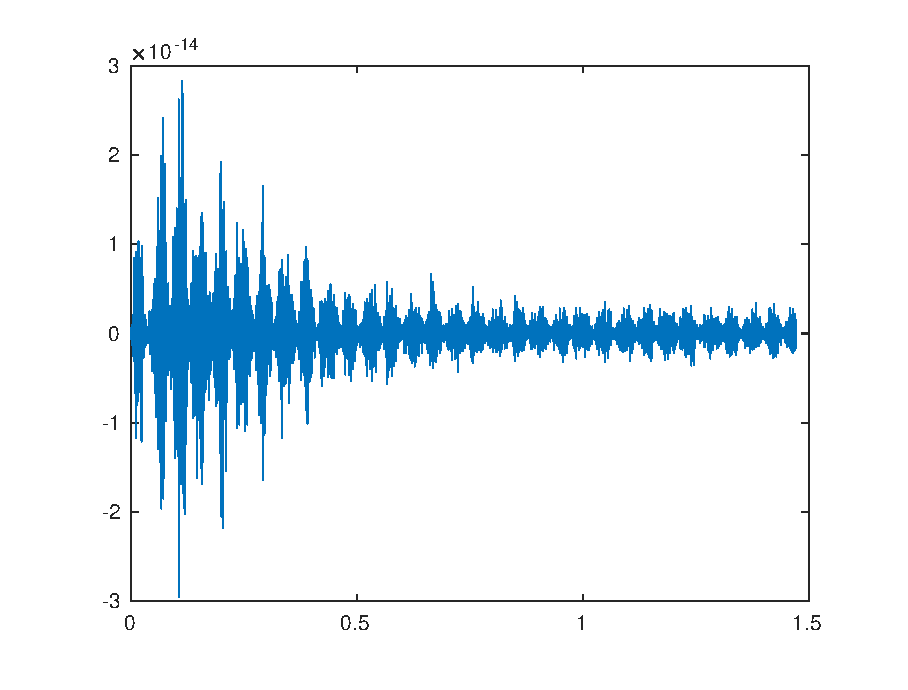
\includegraphics[width=1.1\textwidth, height=0.52\textwidth]{images/cons_momv.eps}\hfill
        \caption{v-momentum}
        \label{fig:Mass}
    \end{subfigure}
    \hfill
    \begin{subfigure}[b]{0.9\textwidth}
        \centering
        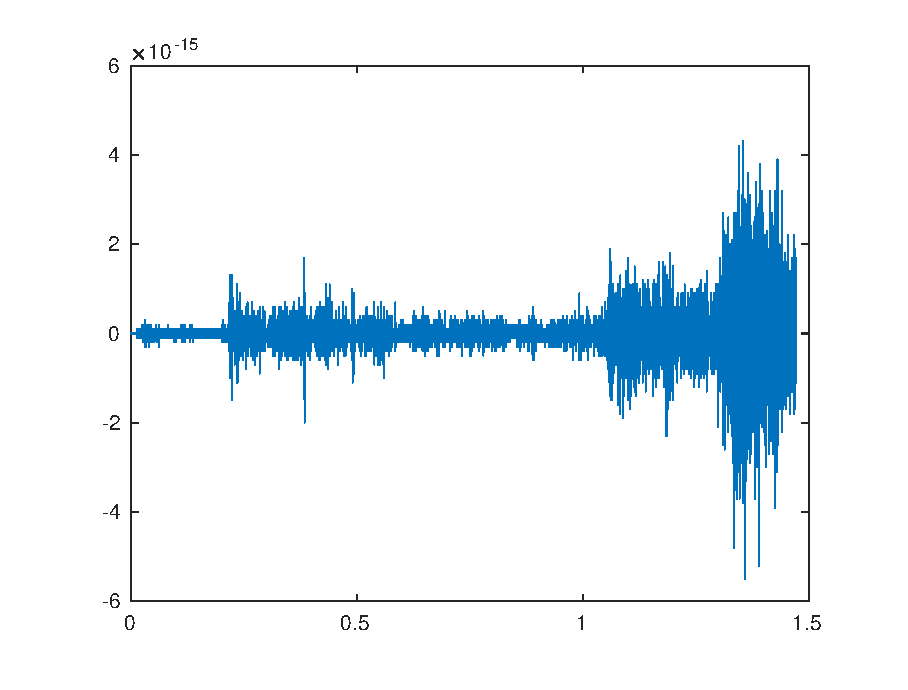
\includegraphics[width=1.1\textwidth,height=0.52\textwidth]{images/cons_vort.eps}\hfill
        \caption{vorticity}
        \label{Momentum}
    \end{subfigure}
    \caption{conservation plots of momentum, vorticity.}
    \label{fig:2Dcons_B}
\end{figure}

We draw the conclusion that the physical quantities mass, momentum, and vorticity (2D only) are adequetly conserved due to the telescoping nature of the schemes.
But the energy is not adequetly conserved due to the inability of the applied numerical methods to capture solutions in the regions of non-linear shocks \cite{Lax}, and also the 
inherint non-linearity of this quantity. 
